
\documentclass{report}

\usepackage[utf8]{inputenc}
\usepackage[italian]{babel}
\usepackage{import}
\usepackage{todonotes}
\usepackage{color}
\usepackage{rotating}
\usepackage[hidelinks]{hyperref}
\usepackage{url}
\usepackage{pdfpages}
\usepackage{siunitx}
\usepackage{pdflscape}
\usepackage{subfig}
\usepackage[euler]{textgreek}
\usepackage{mhchem}

\usepackage{multirow}

\usepackage{enumerate} 
\usepackage{amsmath}
\usepackage{amsfonts}

\usepackage[signatures,swapnames,sans]{frontespizio}

\usepackage{geometry}
\geometry{portrait, margin=3cm}
\usepackage{siunitx}
\usepackage{booktabs}

\renewcommand*\figurename{Figura}

\newcommand{\sub}[1]{\textsubscript{#1}}
\newcommand{\super}[1]{\textsuperscript{#1}}
\newcommand{\parallelsum}{\mathbin{\!/\mkern-5mu/\!}}

\newcommand{\Fig}[0]{Fig.}

\usepackage{titlesec}

\titleformat{\chapter}{\normalfont\huge}{}{20pt}{\huge\bfseries}

\linespread{1.3}


%% COMANDI UTILI
%\begin{table}[h]
%	\centering
%	\begin{tabular}{|c|c|c|}
%	\cline{2-3} 
%	\multicolumn{1}{c|}{} & \textbf{Valore nominale} & \textbf{Valore misurato}\\ 
%		%\hline
%		%{} & \textbf{Valore nominale} & \textbf{Valore misurato} \\ 
%		\hline
%		$\mathbf{R_1}$ & \SI{18}{k\ohm} & \SI{17.977}{k\ohm} \\ 
%		\hline
%		$\mathbf{R_2}$& \SI{1.8}{k\ohm} & \SI{1.815}{k\ohm} \\ 
%		\hline
%	\end{tabular}
%\caption{Misure delle resistenze utilizzate per il circuito.}
%\label{table:mis_res}
%\end{table}
%\begin{figure}[h!]
%\centering
%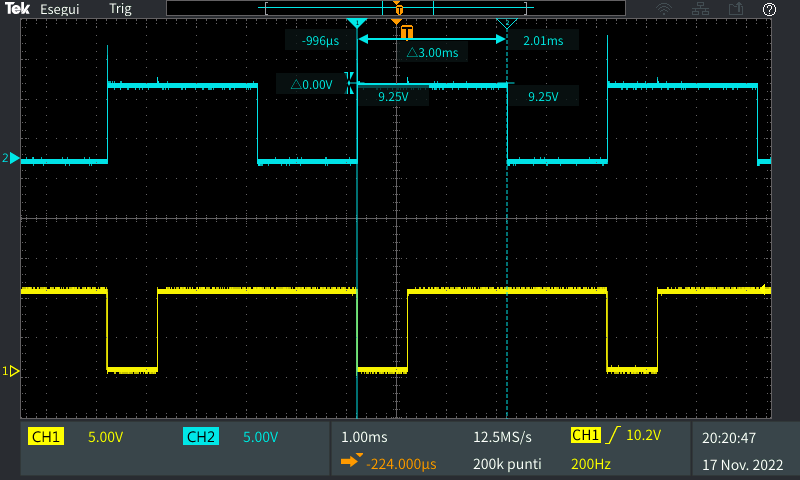
\includegraphics[height=6.5cm]{immagini/TEK00018}\\(a)\\[1ex]
%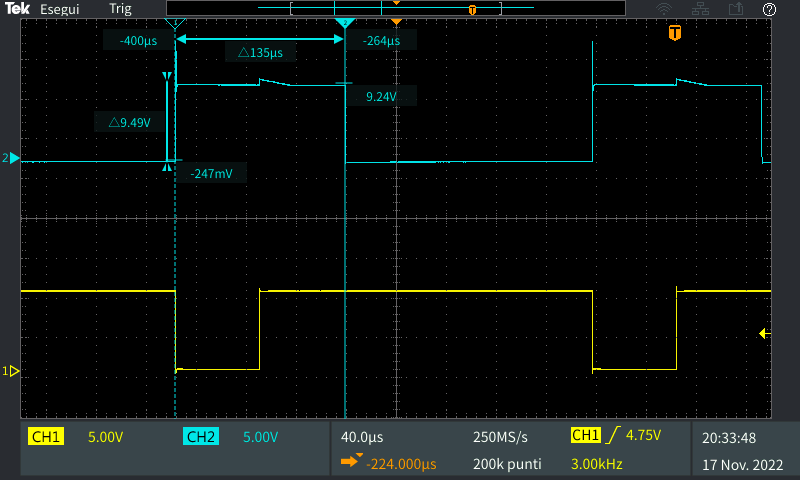
\includegraphics[height=6.5cm]{immagini/TEK00019}\\(b)
%\caption{Risposta del circuito con accoppiamento DC (a) e accoppiamento AC (b).}
%	\label{figura:accopp}
%\end{figure}

\begin{document}
\addtocounter{chapter}{+3}
	\begin{frontespizio}
		\Margini{3cm}{3cm}{3cm}{3cm}
		\Universita{Bergamo}
		\Logo[43.332mm]{unibg-mark}
		\Divisione{Scuola di Ingegneria}
		\Corso[Laurea Magistrale]{Ingegneria Informatica}
		\Titolo{Laboratorio di Elettronica}
		\Sottotitolo{Relazione esperienza di laboratorio 4}
		\Punteggiatura{}
		\NRelatore{Prof.}{Prof.}
		\Relatore{Luigi Gaioni}
		\Candidato[1058231]{Giulia Allievi}
		\Candidato[1059640]{Martina Fanton}
		\Annoaccademico{2022--2023}
		\begin{Preambolo*}
			\usepackage[italian]{babel}
			\usepackage[T1]{fontenc}
			\usepackage[utf8]{inputenc}
			\usepackage{microtype}
			\usepackage{lmodern}
			\graphicspath{{img/}}
			
			\renewcommand{\frontinstitutionfont}{\fontsize{14}{17}\bfseries\scshape}
			\renewcommand{\fronttitlefont}{\fontsize{17}{21}\bfseries\scshape}
			\renewcommand{\frontfootfont}{\fontsize{12}{14}\bfseries\scshape}
		\end{Preambolo*}
	\end{frontespizio}

%----------------------------------------------------------------------------------------
%	PAGINA BIANCA
%----------------------------------------------------------------------------------------
\newpage
\null
\thispagestyle{empty}
\newpage

%----------------------------------------------------------------------------------------
%	INTRO
%----------------------------------------------------------------------------------------
\chapter{Relazione attività di laboratorio 4}
\section*{Introduzione}
Nei circuiti analizzati durante questo laboratorio sono presenti diodi, amplificatori operazionali e un nuovo circuito integrato, il timer 555.\par
Nella figura \ref{figura:timer1} a sinistra, si può vedere la numerazione e la denominazione di ciascun pin di questo componente. Per capire quali sono i terminali, sul package è presente una mezza luna in corrispondenza del pin numero 1 e poi la numerazione prosegue in senso antiorario. Invece nella stessa figura a destra si possono notare i componenti interni di questo circuito integrato e in particolare della tipologia di timer LM555, ovvero quella che abbiamo utilizzato durante questo laboratorio.
\begin{figure}[h!]
	\centering
	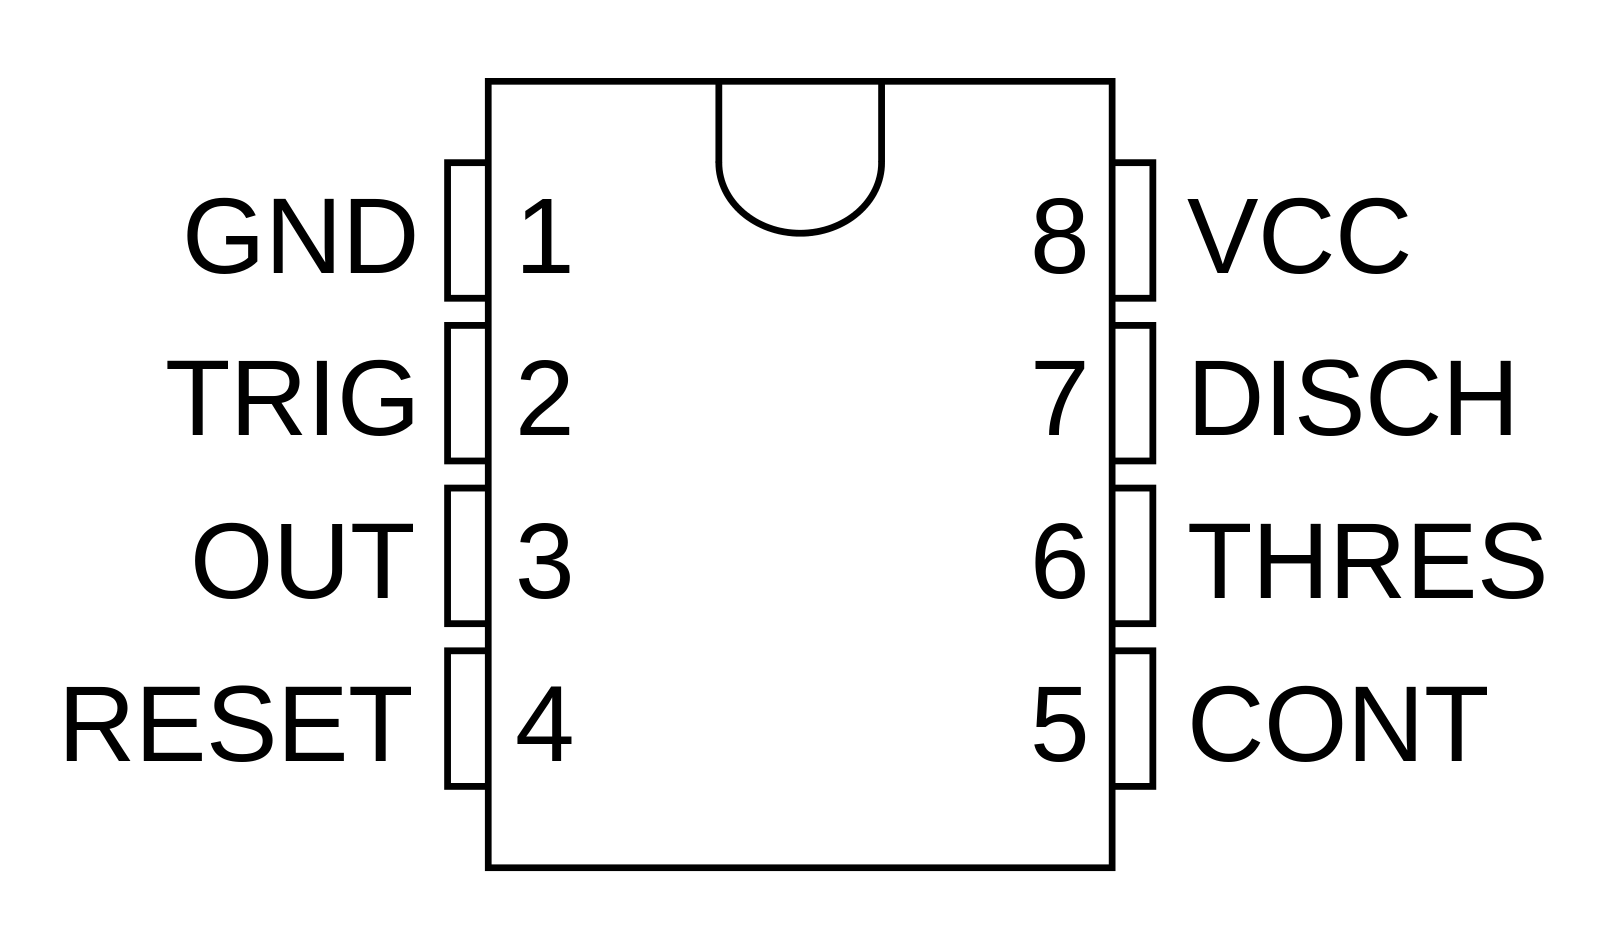
\includegraphics[height=4.6cm]{immagini/timer1}
	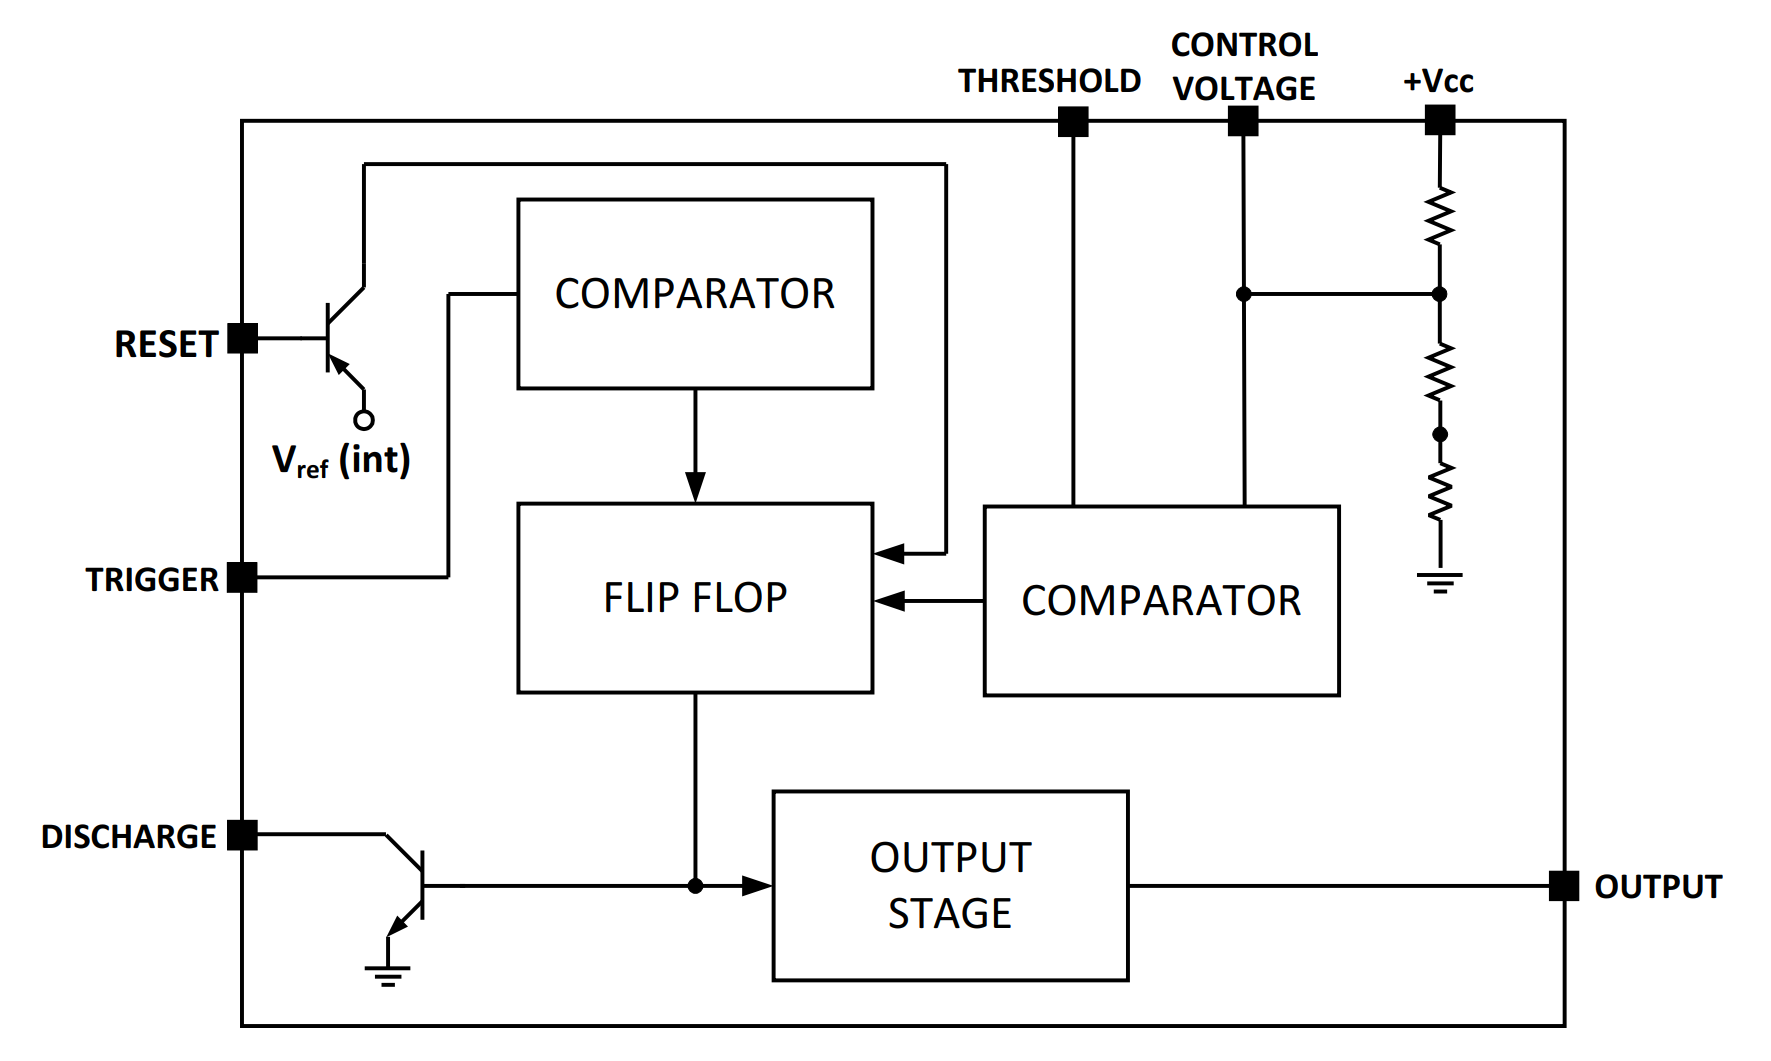
\includegraphics[height=4.6cm]{immagini/timer2}
	\caption{Package (a sinistra) e contenuto (a destra, fonte: \textcolor{blue}{\underline{\href{https://www.ti.com/lit/ds/symlink/lm555.pdf?ts=1667144089940&ref_url=https\%253A\%252F\%252Fwww.ti.com\%252Fproduct\%252FLM555}{datasheet}}} del LM555) del timer 555.}
	\label{figura:timer1}
\end{figure}
\\Questo componente richiede un'alimentazione singola per poter funzionare correttamente: va collegata la tensione positiva $\mathrm{V_{CC}}$ al pin 8, mentre la massa al pin 1.\par
Il timer 555 può essere utilizzato in due configurazioni: astabile oppure monostabile. In questo laboratorio abbiamo utilizzato la seconda configurazione, che è rappresentata nella figura \ref{figura:timer2}.
\begin{figure}[h!]
	\centering
	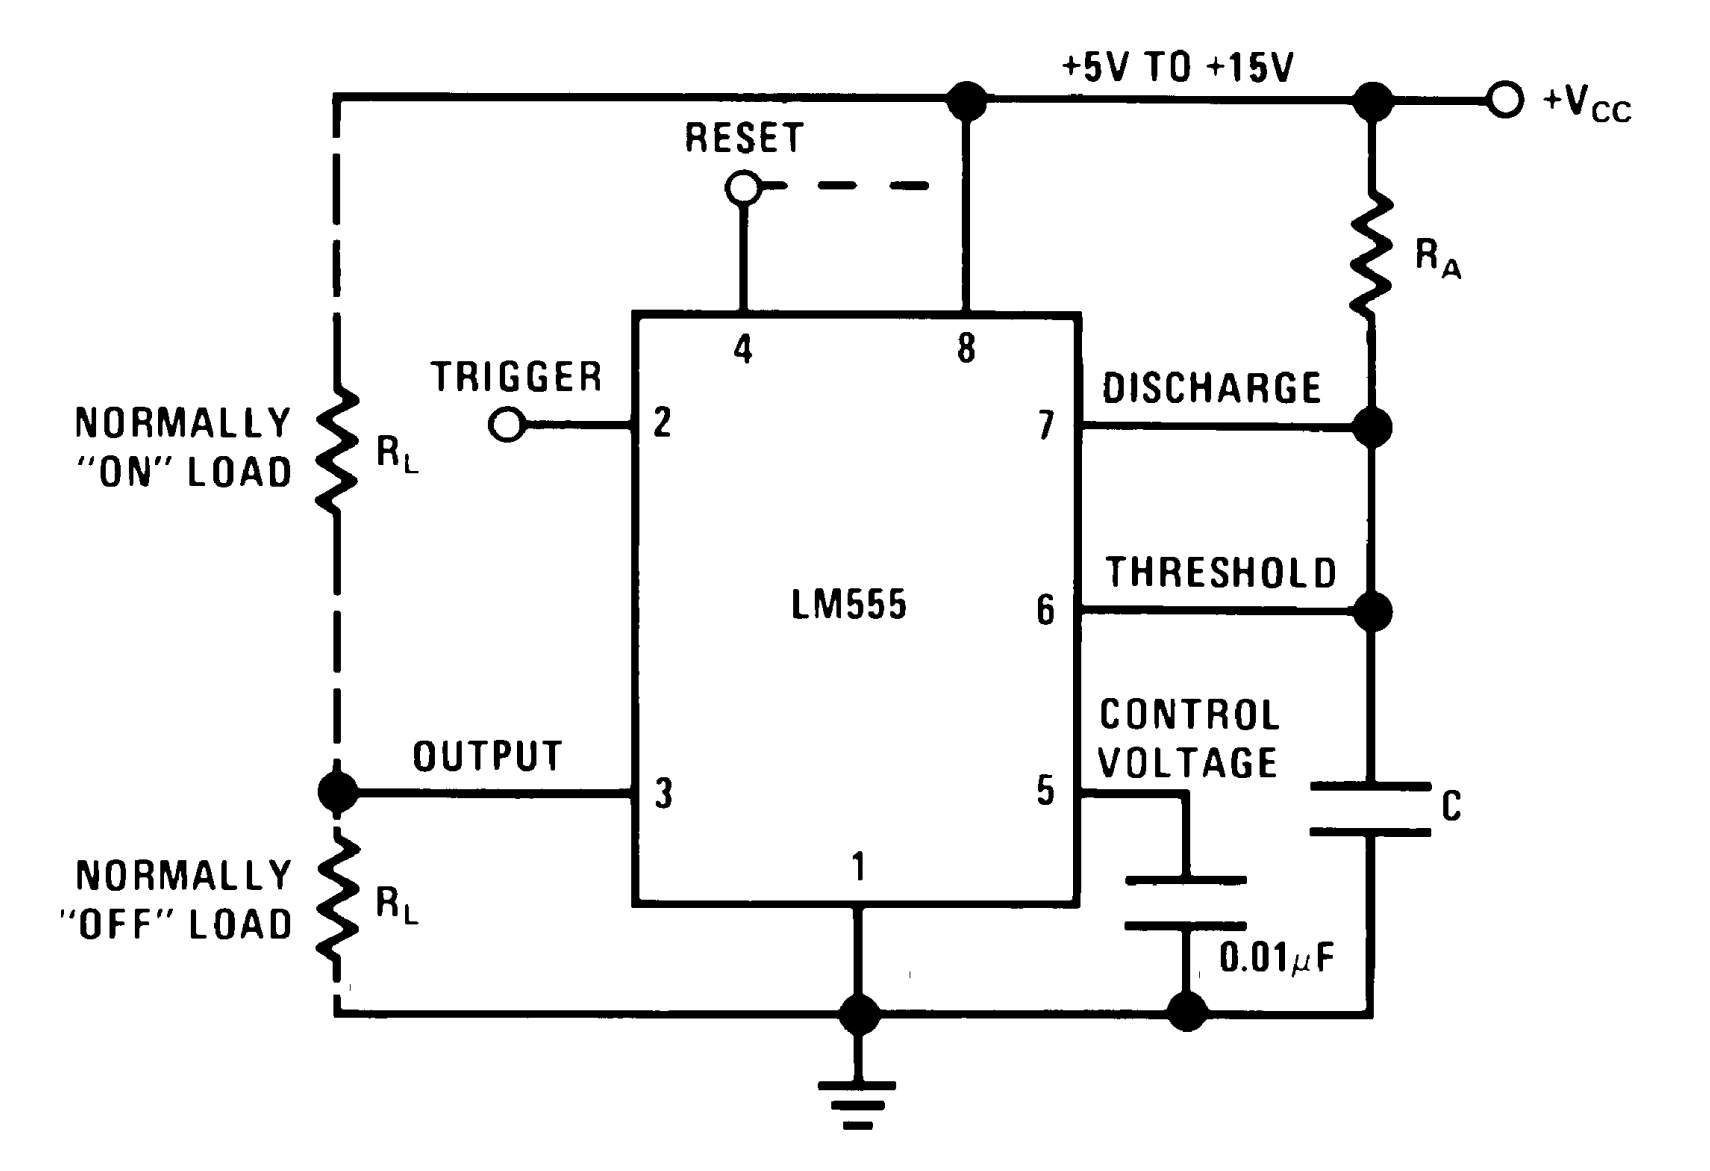
\includegraphics[height=4.6cm]{immagini/timer3}
	\caption{Configurazione monostabile del timer LM555 (fonte: \textcolor{blue}{\underline{\href{https://www.ti.com/lit/ds/symlink/lm555.pdf?ts=1667144089940&ref_url=https\%253A\%252F\%252Fwww.ti.com\%252Fproduct\%252FLM555}{datasheet}}} del LM555).}
	\label{figura:timer2}
\end{figure}

\newpage
\section{Circuito 1: circuito monostabile con trigger di Schmitt}
\subsection{Schema del circuito e Funzione di Trasferimento}
Questo circuito (in figura \ref{figura:schema1}) è stato ottenuto apportando delle modifiche all'oscillatore analizzato nel precedente laboratorio. In particolare sono stati aggiunti un diodo (con il catodo collegato a massa e con l'anodo collegato alla reazione negativa) e una rete di filtraggio (situata all'ingresso non invertente dell'amplificatore e collegata al circuito tramite un ulteriore diodo). Entrambi i diodi utilizzati sono di tipo 1N4148.\par
Per riuscire a visualizzare correttamente tutti i segnali sull'oscilloscopio, abbiamo sostituito l'amplificatore \textmu A741 utilizzato nei precedenti laboratori con un OPAMP di tipo TL071, perché abbiamo osservato sperimentalmente che era più performante per questo particolare circuito.
\begin{figure}[h!]
	\centering
	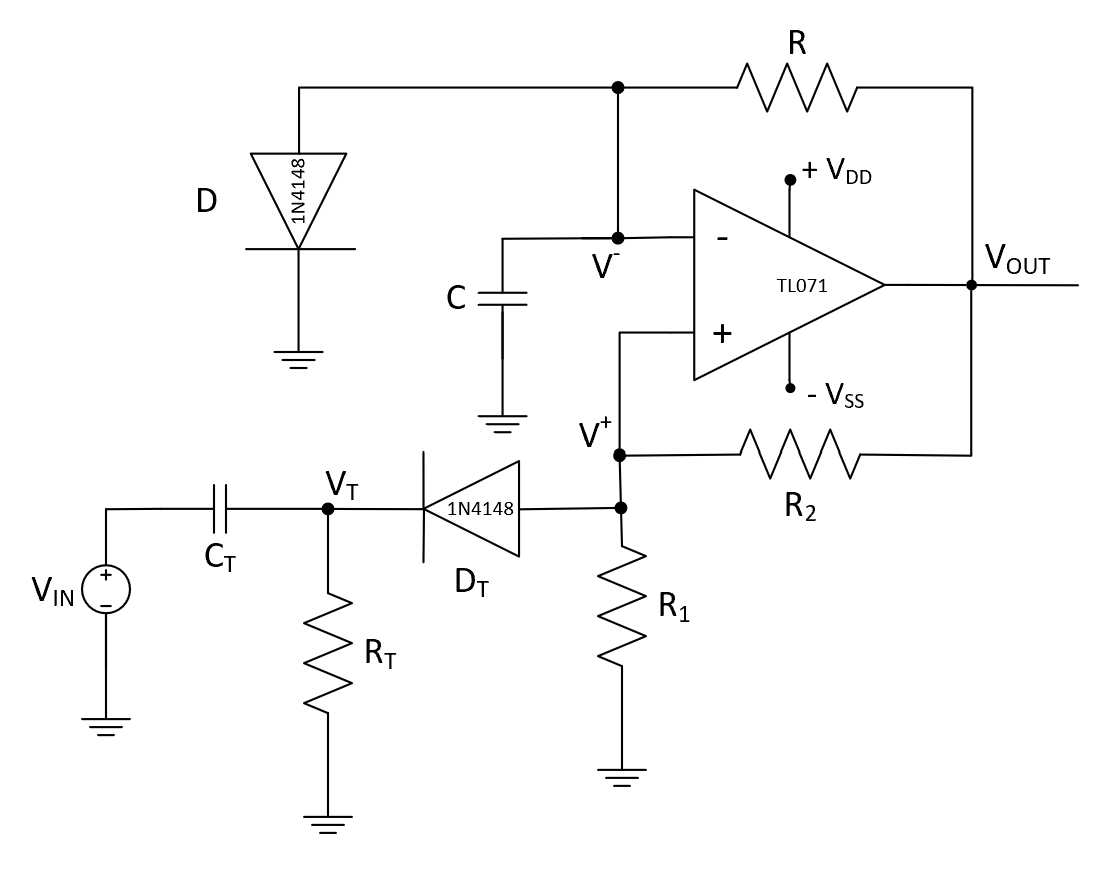
\includegraphics[height=7.5cm]{immagini/schema1}
	\caption{Schema del circuito monostabile con trigger di Schmitt.}
	\label{figura:schema1}
\end{figure}
\\\` E un circuito \textit{monostabile} (detto anche \textit{one-shot}) perché presenta uno stato stabile, ovvero quello in cui la tensione di uscita $\displaystyle\mathrm{V_{OUT}}$ si trova a un valore pari a $\displaystyle\mathrm{V_{DD}}$, ma può andare allo stato instabile in seguito ad uno stimolo esterno ed in uscita si avrà un impulso negativo fino a $\displaystyle\mathrm{V_{SS}}$ con una durata definita.  Questa durata dipende dal processo di \todo{scarica?}{carica} del condensatore verso il valore di $\displaystyle\mathrm{V_{SS}}$ e questo processo viene interrotto quando viene raggiunta la soglia $\displaystyle\mathrm{V_L^+}$. Difatti la tensione sul condensatore può essere calcolata come:
\\[4pt]\indent$\displaystyle{\mathrm{V_C(t)}=\mathrm{V^-(t)}=\mathrm{V_{SS}}+(0.7-\mathrm{V_{SS}}) \cdot e^{-\frac{t-t_0}{\tau}}}$
\\[2pt]dove $\mathrm{t_0}$ è l'istante in cui si ha il fronte di discesa del segnale in ingresso $\mathrm{V_{IN}}$ e l'inizio del processo di \todo{scarica}{carica} del condensatore verso il valore $\mathrm{V_{SS}}$, mentre $\mathrm{\tau}$ corrisponde alla costante di tempo data da: \\\indent$\displaystyle{\mathrm{\tau}= R \cdot C}$.
\\Da questa equazione si può ricavare la formula della durata dell'impulso negativo in uscita, \todo{controlla}{sostituendo a $t$ la durata dell'impulso ($T_A$)}:
\\[4pt]\indent$\displaystyle{T_A=\tau\cdot\ln\biggl(1+\frac{R_2}{R_1}\biggr)\indent \mathrm{se\;}|V_{SS}|\gg\SI{0.7}{\volt}}$
\\[4pt]Terminato quest'intervallo di tempo, il circuito ritornerà automaticamente dallo stato instabile al suo stato stabile. Il circuito rimane al suo stato stabile fin quando non sarà nuovamente perturbato dall'esterno. I circuiti monostabili sono utili per realizzare dei temporizzatori.
\subsection{Analisi e dati sperimentali}
Per poter costruire il circuito sulla breadboard, per prima cosa sono stati scelti i valori dei componenti da utilizzare. Nel caso delle resistenze, le loro misure sono state riportate nella tabella \ref{table:mis_res1}, mentre per i condensatori sono state utilizzate delle capacità di valore nominale di \SI{150}{n\farad} per C e di \SI{1}{n\farad} per $\mathrm{C_T}$. La fotografia del circuito è mostrata in figura \ref{figura:circuito1}.
\begin{table}[h!]
	\centering
	\begin{tabular}{|c|c|c|}
		\cline{2-3} 
		\multicolumn{1}{c|}{} & \textbf{Valore nominale} & \textbf{Valore misurato}\\ 
		\hline
		$\mathbf{R}$ & \SI{12}{k\ohm} & \SI{11.882}{k\ohm} \\ 
		\hline
		$\mathbf{R_1}$ & \SI{12}{k\ohm} & \SI{11.934}{k\ohm} \\ 
		\hline
		$\mathbf{R_2}$ & \SI{12}{k\ohm} & \SI{11.950}{k\ohm} \\ 
		\hline
		$\mathbf{R_T}$ & \SI{12}{k\ohm} & \SI{11.894}{k\ohm} \\ 
		\hline
	\end{tabular}
	\caption{Misure delle resistenze utilizzate per il circuito.}
	\label{table:mis_res1}
\end{table}
\\Una volta costruito il circuito (figura \ref{figura:circuito1}), è stato alimentato con una tensione duale di $\mathrm{\pm\SI{10}{\volt}}$ e poi gli è stato fornito in ingresso un segnale a onda quadra (detto segnale di trigger) con duty cycle del 20\% e frequenza di \SI{100}{\hertz}. Abbiamo scelto il valore di duty cycle più piccolo che il generatore di forme d'onda può erogare perché nell'intervallo di tempo in cui l'onda quadra è bassa, il condensatore deve scaricarsi fino a $\mathrm{V_L^+}$ e quindi caricarsi fino a +\SI{0.7}{\volt}. Dato che tutto questo non avviene istantaneamente, ma ad una velocità legata a $\tau$, affinché il circuito funzioni correttamente è necessario che l'onda quadra stia al livello logico basso per un tempo sufficiente. La tensione picco-picco utilizzata è di \SI{10}{\volt} con offset DC di ???.
\begin{figure}[h!]
	\centering
	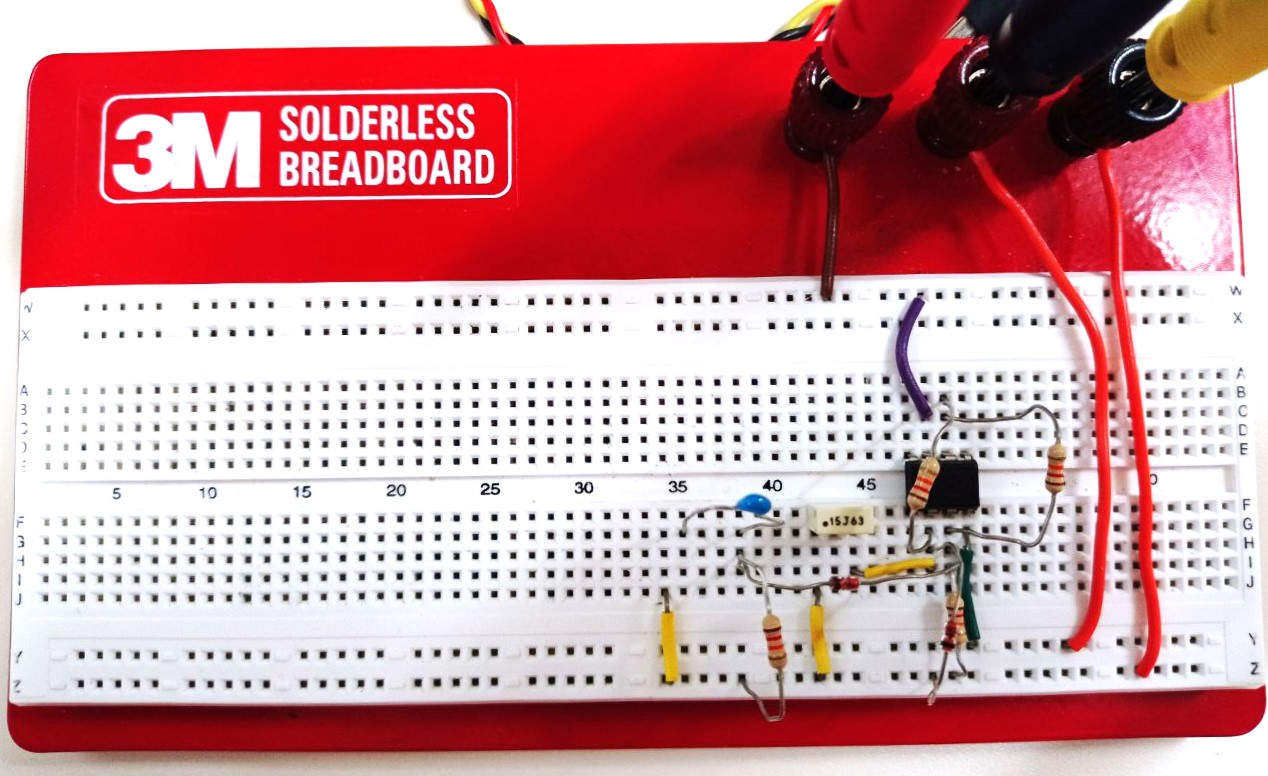
\includegraphics[height=6.5cm]{immagini/circuito1}
	\caption{Fotografia del circuito monostabile con trigger di Schmitt realizzato in laboratorio.}
	\label{figura:circuito1}
\end{figure}
\\Nella figura \ref{figura:TEK00002} sono mostrati il segnale in ingresso $\mathrm{V_{IN}}$ (in giallo, CH1) e il segnale in uscita $\mathrm{V_{OUT}}$ (in azzurro, CH2). \`E stata effettuata anche la misura di $\mathrm{T_A}$ utilizzando i cursori dell'oscilloscopio, così da poterla confrontare con il risultato teorico.
%%% TODO1: rifare screen oscilloscopio con cursori giusti
\begin{figure}[h!]
	\centering
	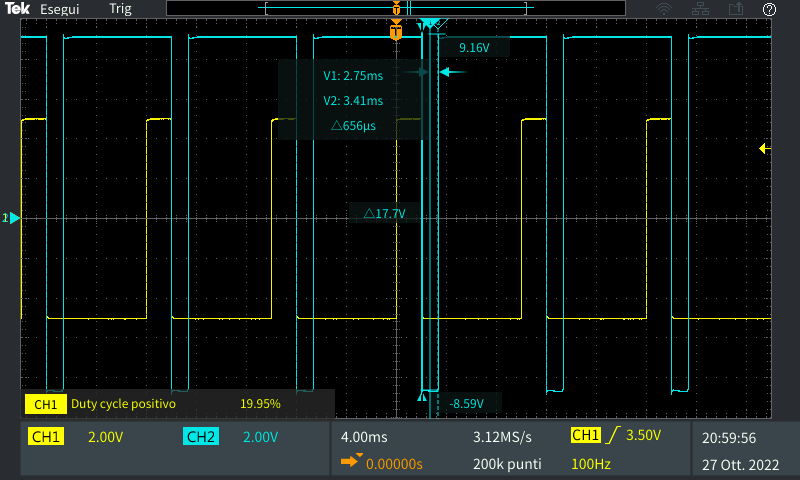
\includegraphics[height=6cm]{immagini/TEK00002}
	\caption{Confronto di $\mathrm{V_{IN}}$ (CH1) con $\mathrm{V_{OUT}}$ (CH2) e misura di $\mathrm{T_A}$ con cursori.}
	\label{figura:TEK00002}
\end{figure}
\\Successivamente, abbiamo utilizzato le formule descritte nella sezione precedente per verificare la correttezza della misura della durata dell'impulso negativo in uscita ($\mathrm{T_A}$) ottenuta con l'oscilloscopio:
\\[4pt]\indent$\displaystyle{T_A=\tau\cdot\ln\biggl(1+\frac{R_2}{R_1}\biggr)=\SI{1.8}{m\second}\cdot\ln\biggl(1+\frac{\SI{12}{k\ohm}}{\SI{12}{k\ohm}}\biggr)=\SI{1.248}{m\second}}$
\\[4pt]\indent con $\displaystyle{\tau=R \cdot C=\SI{12}{k\ohm}\cdot\SI{150}{n\farad}=\SI{1.8}{m\second}}$
\\[4pt]La verifica è quindi soddisfatta perché l'oscilloscopio misura una durata dell'impulso di \SI{1.312}{m\second}, dunque l'errore tra i due valori è circa del 4\%. Questa percentuale di errore è causata in parte anche dall'imprecisione  della strumentazione utilizzata. Infatti, con il generatore di forme d'onda è stata applicata in ingresso un'onda quadra con duty cycle pari al 20\%, mentre l'oscilloscopio ne rileva un valore di 19.95\% (in figura \ref{figura:TEK00002}) e quindi leggermente inferiore. Di conseguenza la rilevazione sull'oscilloscopio di una durata dell'impulso negativo maggiore è determinata dal fatto che l'onda rimane a un livello basso per più tempo rispetto al periodo basso teorico.\par
%%% Correggere in base a nuovo grafico
%% T_B serve solo per il duty cycle?  
Abbiamo poi confrontato la durata dell'impulso negativo in uscita $\mathrm{T_A}$ con la durata dell'impulso negativo in ingresso $\mathrm{T_B}$, calcolata come:
\\[4pt]\indent$\displaystyle{T_B=(1-\delta)\cdot T=(1-20\%)\cdot\SI{10}{m\second}=\SI{8}{m\second}}$
\\[4pt]\indent con f = \SI{100}{\hertz} $\Rightarrow\;\displaystyle{T=\frac{1}{f}=\SI{10}{m\second}}$
\\[4pt]Come ci si aspetta dalla teoria, si ottiene che $\mathrm{T_B}>>\mathrm{T_A}$ perché il duty cycle ha un valore inferiore al 50\% ed è piuttosto piccolo.\par
Terminata l'analisi sulla durata dell'impulso negativo, sono stati confrontati i segnali delle tensioni in ingresso e in uscita rispetto a quelle presenti sugli ingressi dell'OPAMP e a quella presente nel nodo $\mathrm{V_T}$. Riportiamo di seguito i grafici più significativi per l'analisi del circuito.\par
Per quanto riguarda la tensione sull'ingresso non invertente $\mathrm{V^+}$, essa varia tra $\mathrm{V_L^+}$ e $\mathrm{V_H^+}$ e, come si può notare dalla figura \ref{figura:TEK00003}, questi due valori non sono simmetrici. Questo succede perché:
\begin{itemize}
	\item se $\mathrm{V_{OUT}}$ è negativa (ovvero pari a $\mathrm{V_{SS}}$) si ha che il diodo $\mathrm{D_T}$ è spento e quindi:
	\\[4pt]$\displaystyle{\;\;\;V_L^+=\frac{V_{SS}}{2}=\frac{\SI{-10}{\volt}}{2}=\SI{-5}{\volt}}$;
	\item se $\mathrm{V_{OUT}}$ è positiva (ovvero pari a $\mathrm{V_{DD}}$) si ha che il diodo $\mathrm{D_T}$ è accesso e quindi:
	\\[4pt]$\displaystyle{\;\;\;V_H^+=\frac{V_{DD}}{3}=\frac{\SI{10}{\volt}}{3}=\SI{3.33}{\volt}}$.
\end{itemize}
\begin{figure}[h!]
	\centering
	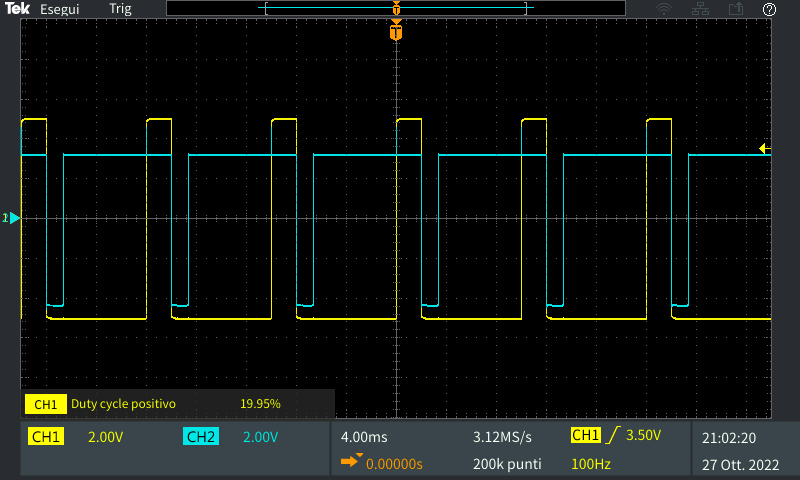
\includegraphics[height=6cm]{immagini/TEK00003}
	\caption{Confronto di $\mathrm{V_{IN}}$ (CH1) con $\mathrm{V^+}$ (CH2).}
	\label{figura:TEK00003}
\end{figure}
%% TODO2: screen v+ e vout
\todo{foto oscilloscopio con V+ e Vout}
Se confrontiamo le tensioni all'ingresso non invertente ed in uscita, vediamo che entrambe hanno lo stesso andamento, ma la tensione $\mathrm{V_{OUT}}$ è limitata dalle alimentazioni mentre la tensione $\mathrm{V^+}$ è limitata dalle due soglie del trigger di Schmitt, $\mathrm{V_L^+}$ e $\mathrm{V_H^+}$.
% mettere grafico
\\(foto)
%%%
\\Invece la tensione sull'ingresso invertente $\mathrm{V^-}$, corrispondente alla tensione sul condensatore C ($\mathrm{V_C}$), è stata rappresentata nella figura \ref{figura:TEK00004e5} e presenta un'espressione nel tempo pari a:
\\[4pt]\indent$\displaystyle{V_C(t)=V^-(t)=V_{SS}+(0.7-V_{SS})\cdot e^{-\frac{t-t_0}{\tau}}=\SI{-10}{\volt}+\SI{10.7}{\volt}\cdot e^{-\frac{t-t_0}{\SI{1.8}{m\second}}}}$
\\Il suo andamento nel tempo è simile a quello di un treno di impulsi negativi.
\todo{determinare valore di t0 da mettere nell'espressione. per me va anche separata carica da scarica perché sono formule diverse}
\begin{figure}[h!]
	\centering
	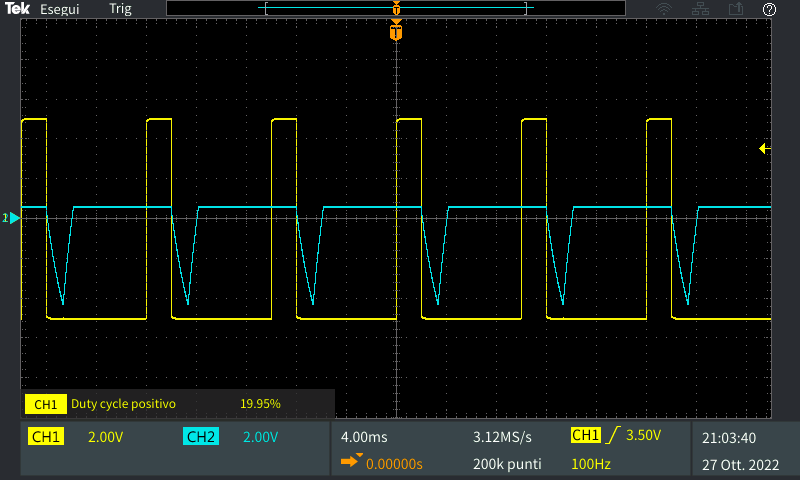
\includegraphics[height=4.6cm]{immagini/TEK00004}
	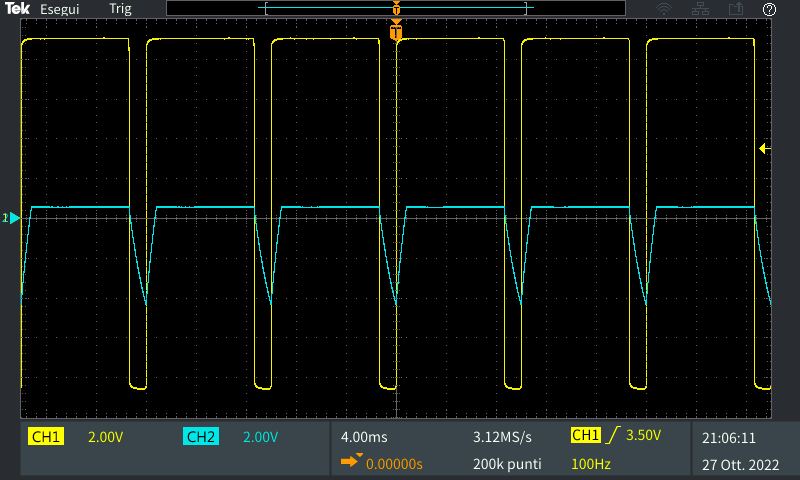
\includegraphics[height=4.6cm]{immagini/TEK00005}
	\caption{Confronto di $\mathrm{V^-}$ (CH2) con $\mathrm{V_{IN}}$ (CH1 a sinistra) e con $\mathrm{V_{OUT}}$ (CH1 a destra).}
	\label{figura:TEK00004e5}
\end{figure}
%% TODO3: derivatore
\\Analizzamo ora le tensioni $\mathrm{V_T}$ e $\mathrm{V_{IN}}$. Il sottocircuito a sinista del diodo $\mathrm{D_T}$ si comporta come un derivatore della tensione in ingresso, a patto di lavorare ad una frequenza molto minore della frequenza di taglio. La frequenza di taglio del filtro è:
\\[4pt]\indent$\displaystyle{f_T = \frac{1}{2\pi\cdot R_T\cdot C_T} = \frac{1}{2\pi\cdot \SI{12}{k\ohm}\cdot\SI{1}{n\farad}} =\SI{13.263}{k\hertz}}$
\\[4pt]Dato che il nostro circuito lavora ad una frequenza di \SI{100}{\hertz}, la condizione $f_T\gg f$ è rispetta, pertanto al nodo $\mathrm{V_T}$ avremo la derivata della tensione del nodo $\mathrm{V_{IN}}$. In figura \ref{figura:} è mostrato l'andamento nel tempo delle due tensioni.
\todo{foto oscilloscopio con VT e Vin e Vout}
\\(foto)
%%%
\\Nella figura successiva, sono mostrate tutte le tensioni che abbiamo misurato in precedenza, ottenute simulando il circuito su un periodo di tempo. Anche su questo grafico possiamo ritrovare tutte le considerazioni fatte per i grafici precedenti, fatta eccezione per l'istante iniziale, perché il simulatore inizializza tutti i nodi a \SI{0}{\volt}. 
\begin{figure}[h!]
	\centering
	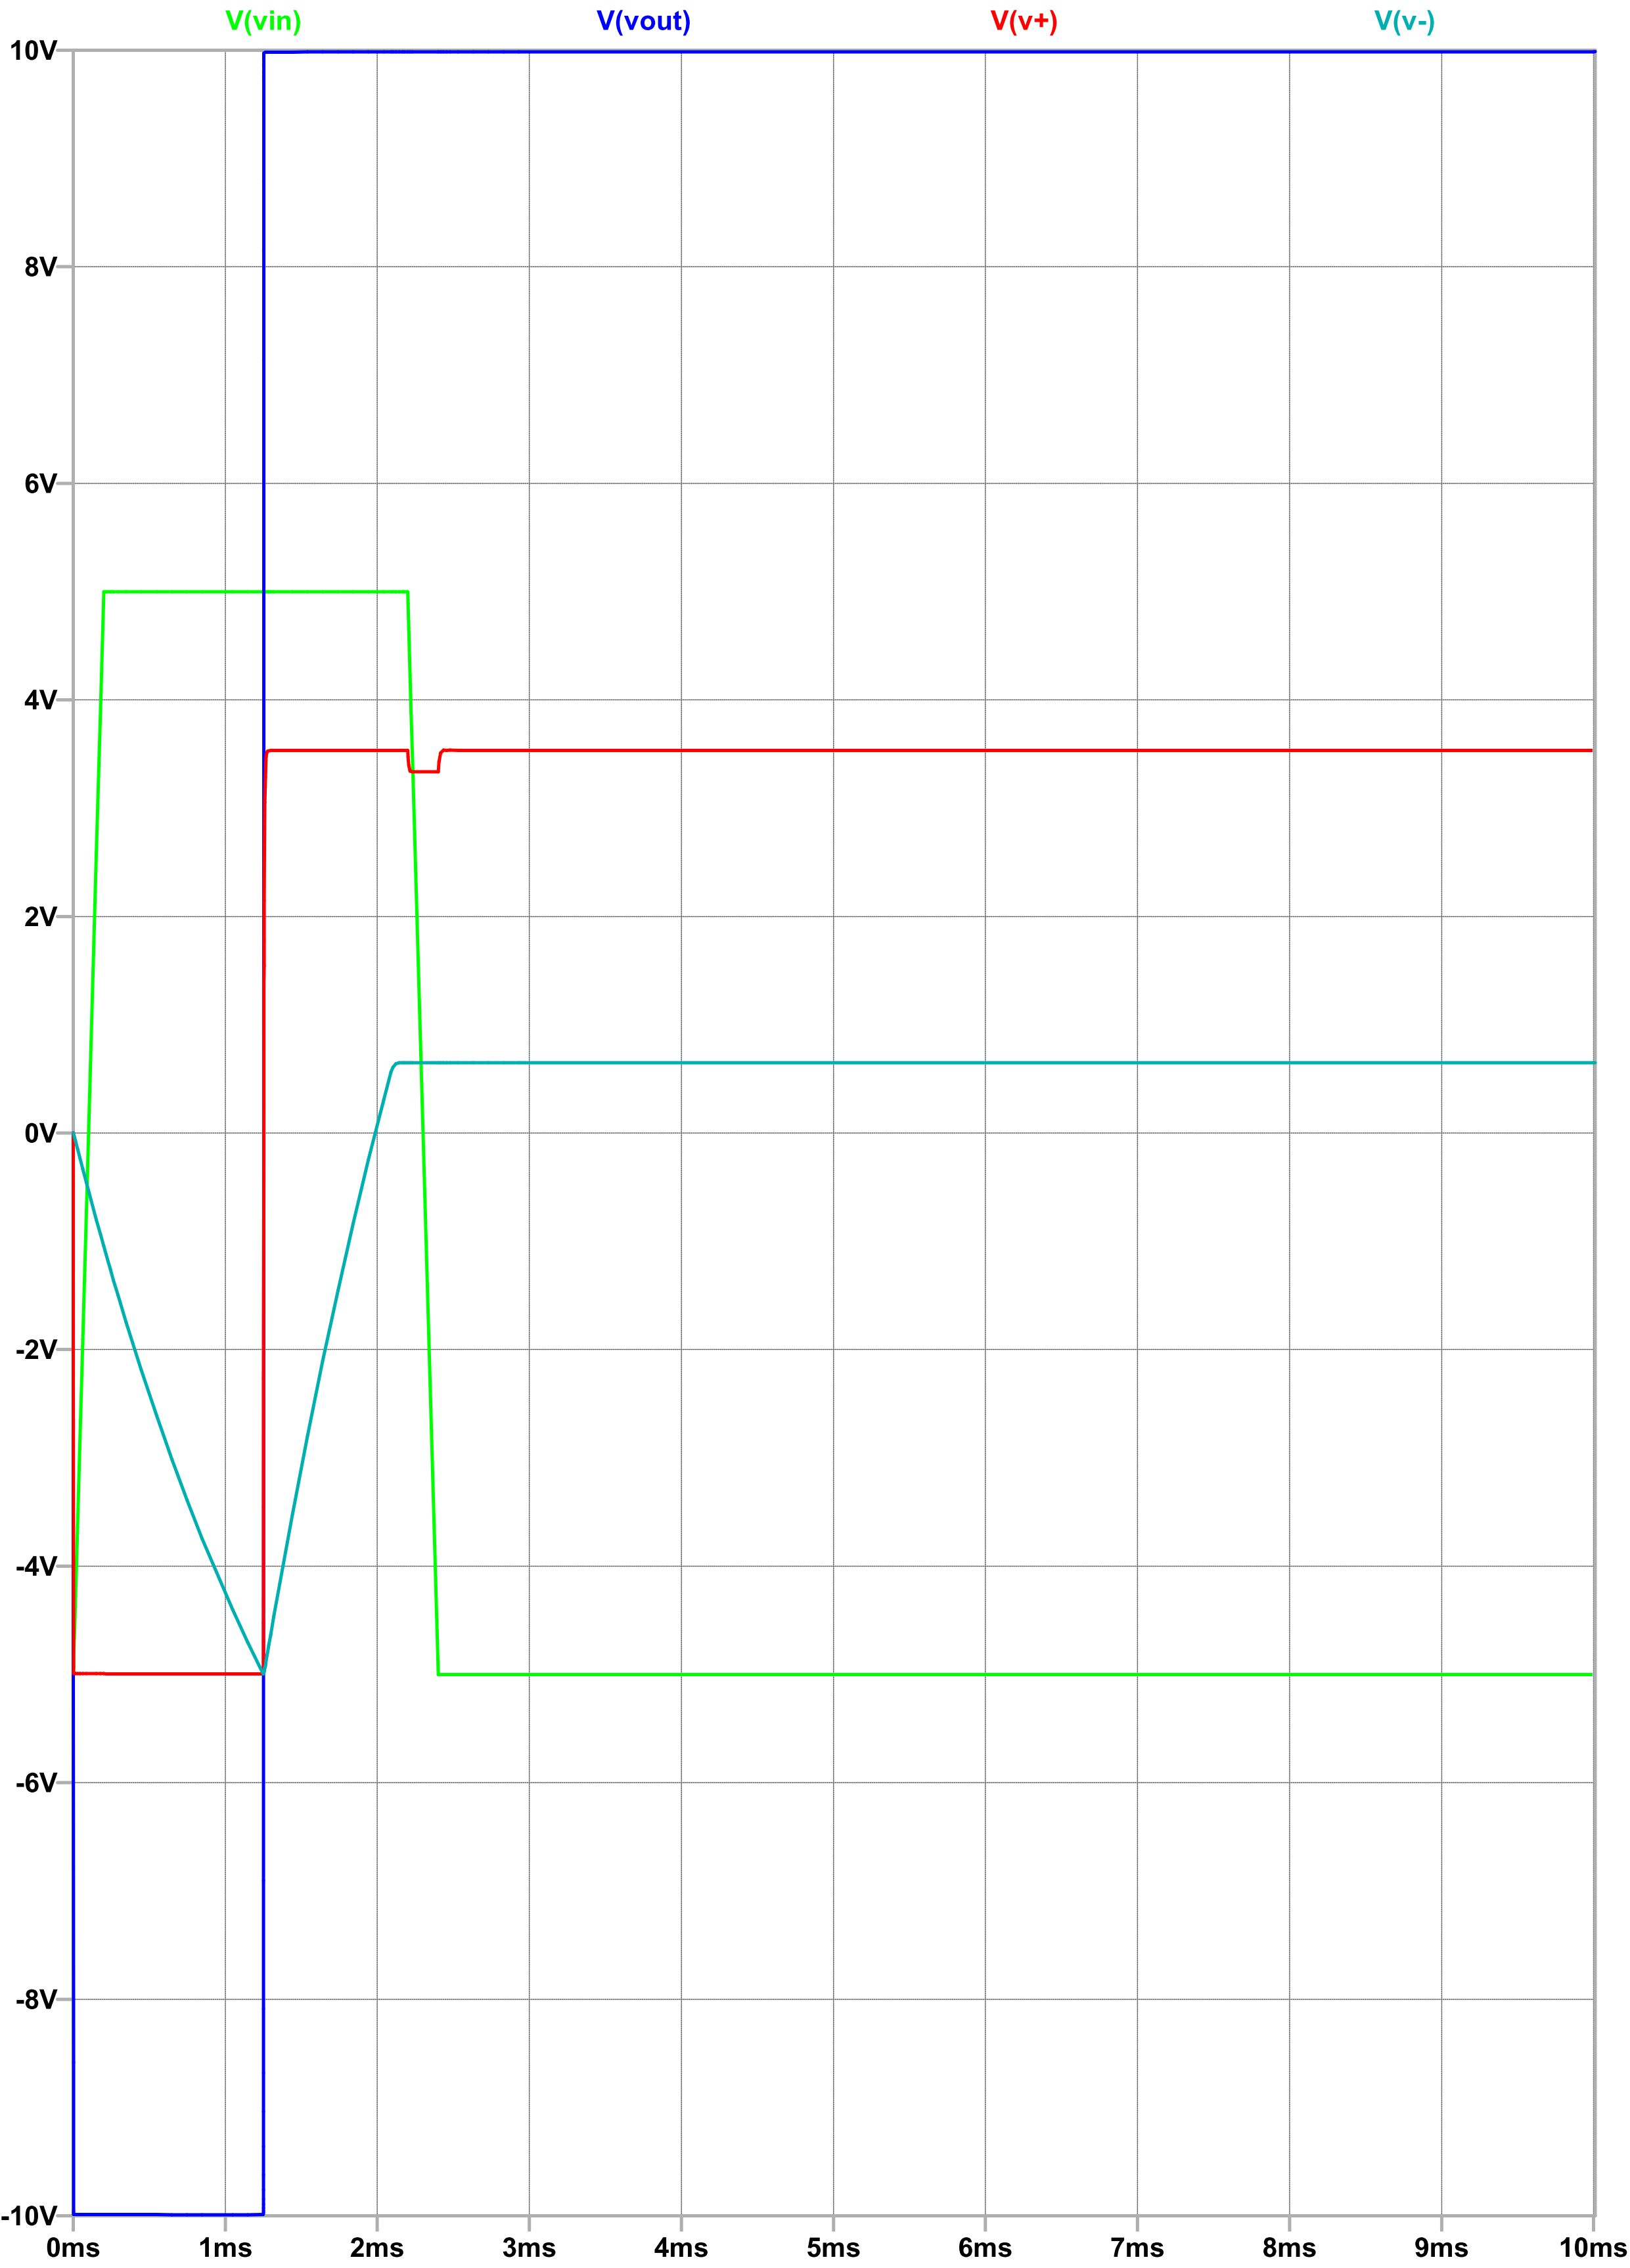
\includegraphics[height=5cm]{immagini/plot_sim} %% va poi ingrandita, messa solo per semplicità impaginazione
	\caption{Confronto di $\mathrm{V_{IN}}$, $\mathrm{V_{OUT}}$, $\mathrm{V^+}$ e $\mathrm{V^-}$.}
	\label{figura:simulazione}
\end{figure}
\\Infine, è stato considerato lo stato stabile di questo circuito, che consiste nell'aggiungere al circuito del precedente laboratorio soltanto il diodo D ottenendo il circuito in figura \ref{figura:schema1stabile}. Per questa analisi sono stati mantenuti invariati i valori dei componenti utilizzati. Inoltre, al circuito risultante non si applica nessun segnale in ingresso.
\begin{figure}[h!]
	\centering
	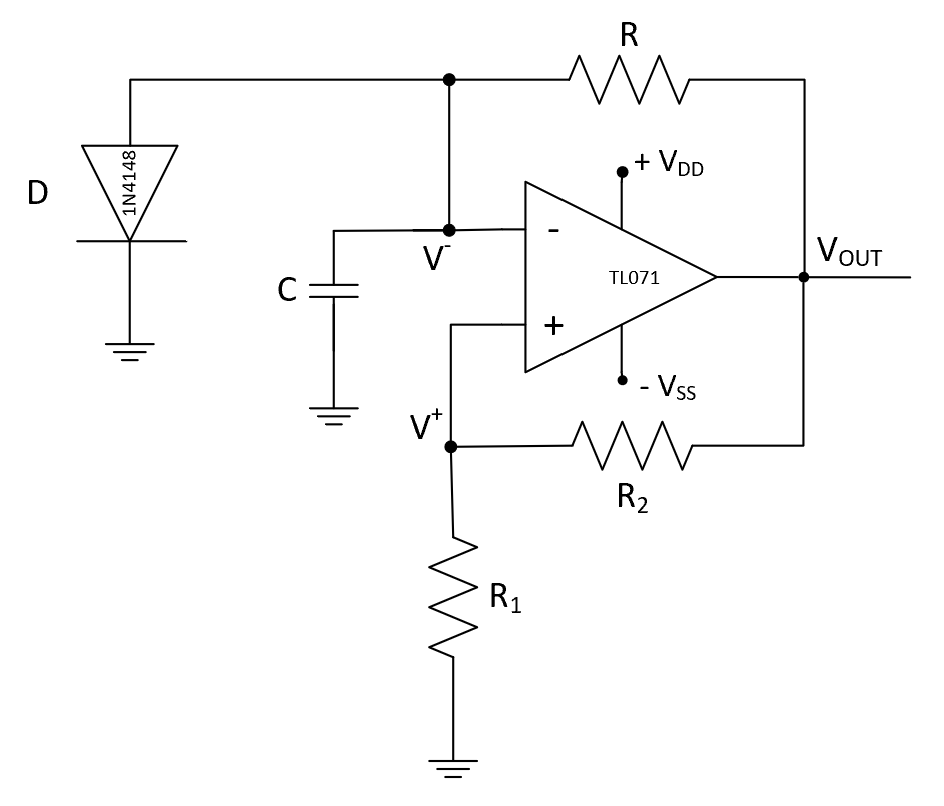
\includegraphics[height=5.5cm]{immagini/schema1stabile}
	\caption{Schema del circuito nello stato stabile.}
	\label{figura:schema1stabile}
\end{figure}
\\Analizzando il segnale sull'ingresso invertente dell'OPAMP, $\mathrm{V^-}$, si può notare che questa tensione (corrispondente alla tensione sul condensatore C), presenta una fase iniziale di carica e poi, una volta raggiunti gli \SI{0.7}{\volt}, viene bloccata poichè è stato raggiunto il valore della tensione ai capi del diodo e quindi esso si accende, impedendo alla capacità di continuare a caricarsi (la corrente che prima fluiva nel condensatore e lo caricava, ora andrà a massa attraverso il diodo acceso). Invece il segnale in uscita, $\mathrm{V_{OUT}}$, rimane al valore dell'alimentazione positiva $\mathrm{V_{DD}}$ e quindi non riesce a commutare, siccome $\mathrm{V^-}$ non riesce mai a superare la soglia $\mathrm{V_H^+}$. Quindi, questo circuito rimane nello stato stabile non oscilla. Il grafico è riportato in figura \ref{figura:simulazione1}. 
\begin{figure}[h!]
	\centering
	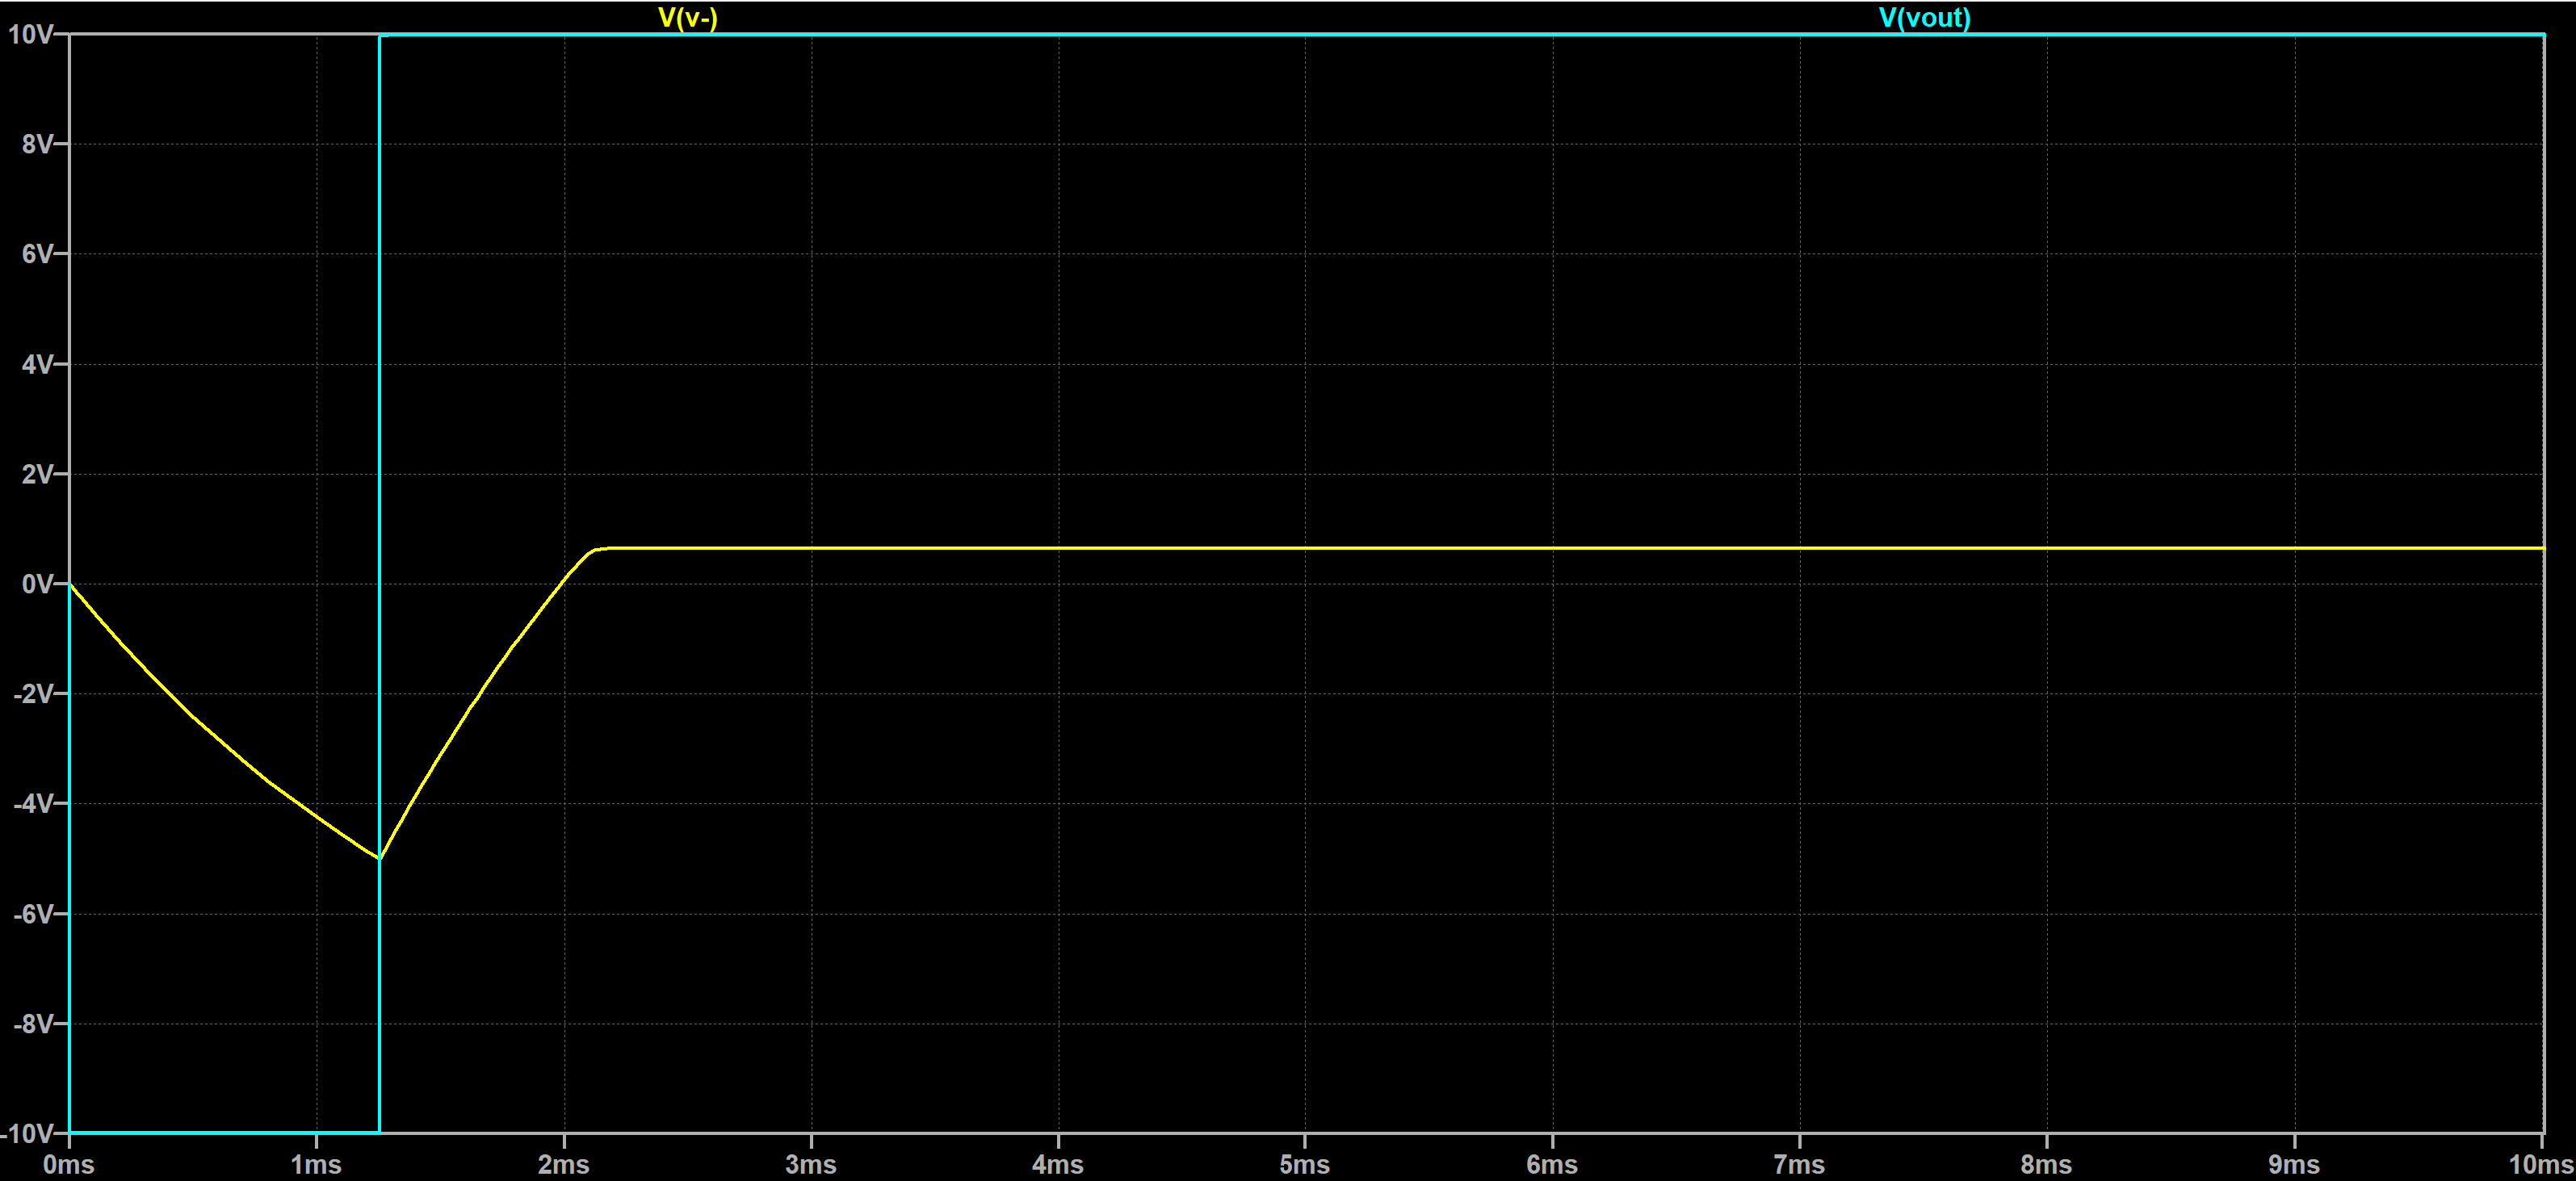
\includegraphics[height=4.6cm]{immagini/plot_sim_stabile}
	\caption{Confronto di $\mathrm{V^-}$ (CH1) con $\mathrm{V_{OUT}}$ (CH2) nello stato stabile.}
	\label{figura:simulazione1}
\end{figure}
\\Per poter rendere questo circuito monostabile, è necessario che la soglia $\mathrm{V_H^+}$ risulti inferiore rispetto a $\mathrm{V^-}$, in modo da avere una transizione su $\mathrm{V_{OUT}}$. Per avere questo effetto è necessario collegare sull'ingresso non invertente dell'OPAMP la rete che funziona come derivatore.
%%% TODO4: ???
\todo{aggiornare foto confronto con oscilloscopio}
%%%

\newpage
\section{Circuito 2: circuito monostabile con NE555}
\subsection{Schema del circuito e Funzione di Trasferimento}
\begin{figure}[h]
	\centering
	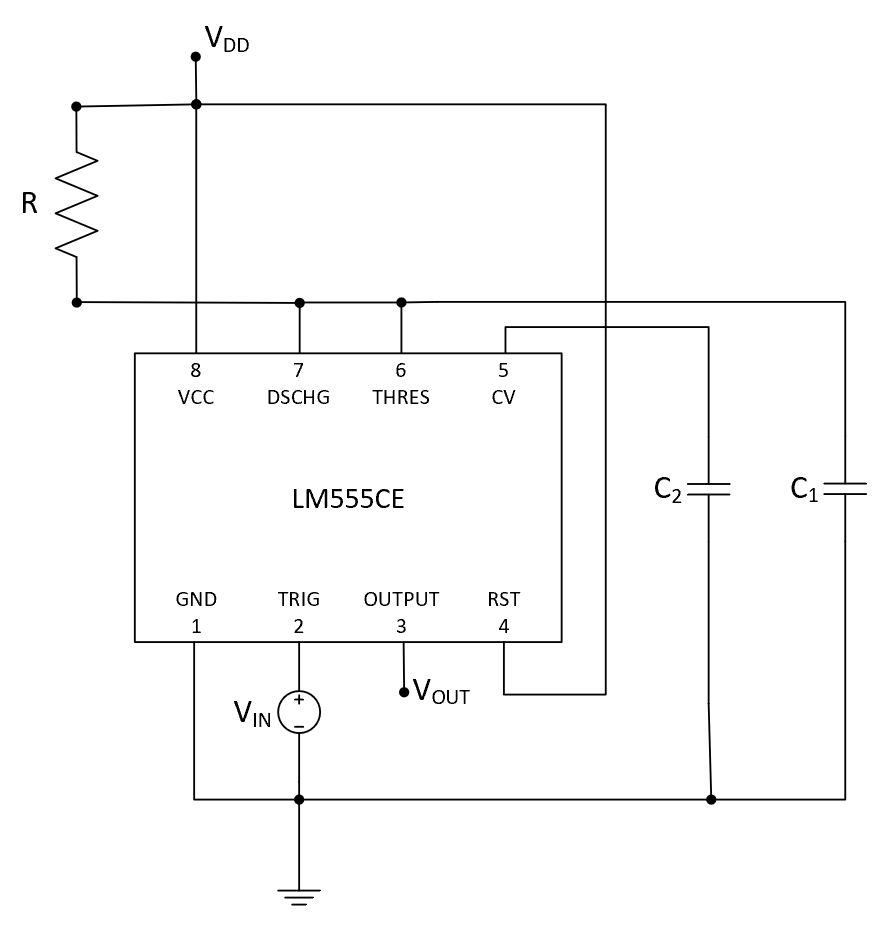
\includegraphics[height=7.5cm]{immagini/schema2}
	\caption{Schema del circuito monostabile con NE555.}
	\label{figura:schema2}
\end{figure}
\subsection{Analisi e dati sperimentali}
%R ... k\ohm --> 12k\ohm
%R 4.698 k\ohm --> 4.7 k\ohm
\begin{figure}[h]
	\centering
	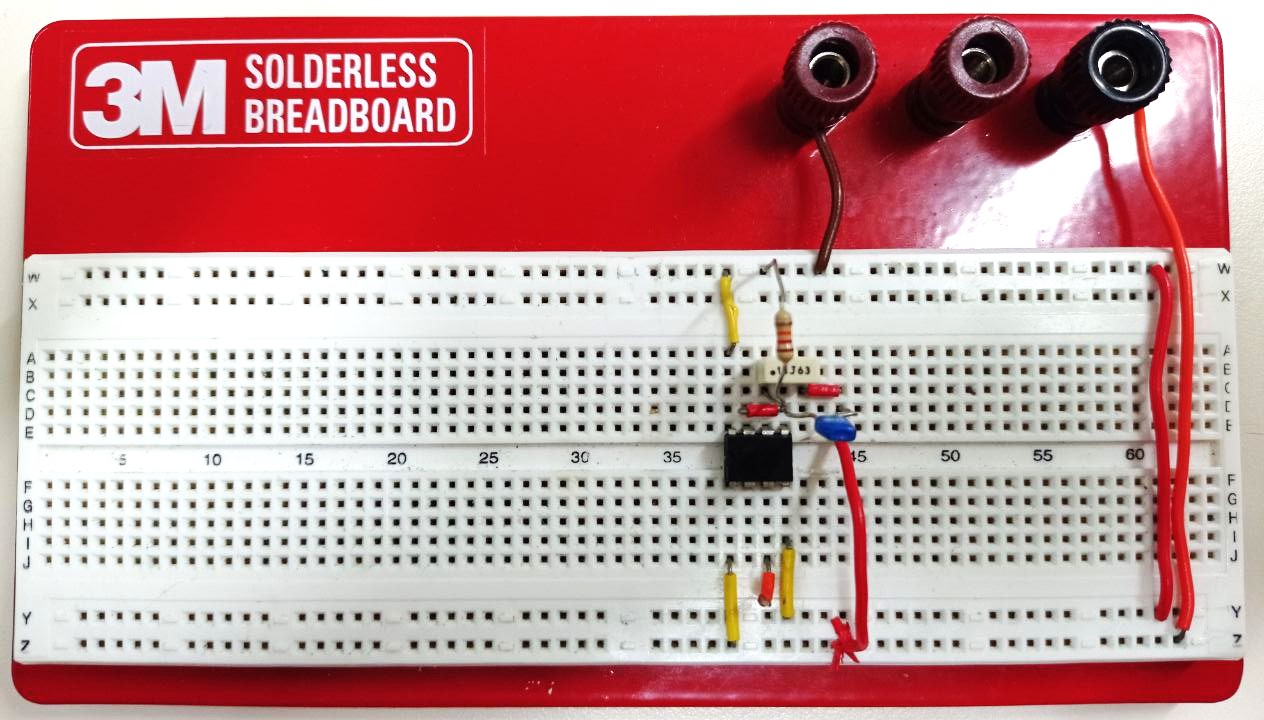
\includegraphics[height=6.5cm]{immagini/circuito2}
	\caption{Fotografia del circuito monostabile con LM555 realizzato in laboratorio.}
	\label{figura:circuito2}
\end{figure}

%----------------------------------------------------------------------------------------

\end{document}
